% ****** Start of file apssamp.tex ******
%
%   This file is part of the APS files in the REVTeX 4.2 distribution.
%   Version 4.2a of REVTeX, December 2014
%
%   Copyright (c) 2014 The American Physical Society.
%
%   See the REVTeX 4 README file for restrictions and more information.
%
% TeX'ing this file requires that you have AMS-LaTeX 2.0 installed
% as well as the rest of the prerequisites for REVTeX 4.2
%
% See the REVTeX 4 README file
% It also requires running BibTeX. The commands are as follows:
%
%  1)  latex apssamp.tex
%  2)  bibtex apssamp
%  3)  latex apssamp.tex
%  4)  latex apssamp.tex
%
\documentclass[%
 reprint,
%superscriptaddress,
%groupedaddress,
%unsortedaddress,
%runinaddress,
%frontmatterverbose, 
%preprint,
%preprintnumbers,
%nofootinbib,
%nobibnotes,
%bibnotes,
 amsmath,amssymb,
 aps,
 pra,
%prb,
%rmp,
%prstab,
%prstper,
%floatfix,
]{revtex4-2}
\usepackage[spanish,es-nodecimaldot]{babel}
\usepackage{color,soul}
\usepackage{physics}
\usepackage{minted}
\usepackage{graphicx}% Include figure files
%\usepackage{svg}
\usepackage{dcolumn}% Align table columns on decimal point
\usepackage{bm}% bold math
\usepackage{hyperref}% add hypertext capabilities
\definecolor{linkcolour}{rgb}{0,0.2,0.6} % Link color
\hypersetup{colorlinks,citecolor=linkcolour,breaklinks,urlcolor=linkcolour,linkcolor=linkcolour}
\usepackage{color,soul}
\usepackage{soulutf8}
\usepackage{mathrsfs}
%\usepackage[mathlines]{lineno}% Enable numbering of text and display math
%\linenumbers\relax % Commence numbering lines

%\usepackage[showframe,%Uncomment any one of the following lines to test 
%%scale=0.7, marginratio={1:1, 2:3}, ignoreall,% default settings
%%text={7in,10in},centering,
%%margin=1.5in,
%%total={6.5in,8.75in}, top=1.2in, left=0.9in, includefoot,
%%height=10in,a5paper,hmargin={3cm,0.8in},
%]{geometry}

\begin{document}

\preprint{APS/123-QED}

\title{Partícula bajo influencia de potencial armónico y anarmónico en colectividad\texorpdfstring{\\}{ }canónica: algoritmos \textit{Matrix Squaring} y \textit{Path Integral}.}% Force line breaks with \\

\author{Juan Esteban Aristizabal Zuluaga}
\affiliation{Instituto de Física, Universidad de Antioquia.}%Lines break automatically or can be forced with \\

\date{\today}% It is always \today, today,
             %  but any date may be explicitly specified

\begin{abstract}
En este artículo presentamos un estudio del oscilador armónico cuántico unidimensional y de un sistema unidimencional de una partícula bajo la acción de un potencial anarmónico, ambos inmersos en un baño térmico. En particular, nos interesamos por la implementación de los algoritomos \textit{Matrix Squaring} y \textit{Path Integral Naive Sampling} que nos permiten obtener informacón relevante de los sistemas en cuestión. Para esto presentamos una breve descripción de los algoritmos así como los resultados obtenidos. En especial, nos enfocamos en calcular la energía promedio de los sistemas y la probabilidad de encontrar a la partícula en una posición dada. Al contrastar los resultados obtenidos con los valores teóricos –cuando es posible– encontramos que ambos algoritmos se aproximan a los valores deseados. Se presenta también la implementación de los algoritmos en el lenguaje de programación «Python». 
\begin{description}
\item[Palabras clave] 	Oscilador armónico, potencial anarmónico, física estadística cuántica, baño\\
térmico, ensamble canónico, \textit{matrix squaring}, \textit{path integral}.
\end{description}
\end{abstract}

%\keywords{Suggested keywords}%Use showkeys class option if keyword
                              %display desired
\maketitle

%\tableofcontents

\section{\label{sec:Intro}Introducción}

El oscilador armónico ha sido históricamente para la física un sistema simple pero del que se puede extraer gran cantidad de información y con el que se han descubierto muchos nuevos métodos y hasta teorías completas, basadas en los razonamientos y el conocimiento obtenido de éste. Por citar un ejemplo, está la cuantización del campo electromagnético que se puede reducir a un sistema «osciladores armónicos» no acoplados y en general las teorías de segunda cuantización en la base número usan gran parte del formalismo del oscilador armónico cuántico, aunque con un significado muy diferente al que se le da en el sistema que nos compete\cite{Grynberg2010,Schwartz2013}. Además, los casos anarmónicos han sido igualmente importantes, ya que muchos sistemas reales se pueden modelar usando este tipo de potenciales, además que éstos se puede estudiar generalmente como una perturbación del potencial armónico. 

En este trabajo estudiamos dos métodos computacionales que permiten obtener información acerca tanto del oscilador armónico unidimensional como de un sistema de una partícula bajo la acción de un potencial anarmónico unidimensional, ambos inmersos en un baño térmico.

El primer método que presentamos se conoce como \textit{Matrix Squaring} y se basa en la convolución de matrices densidad en el ensamble canónico. Cuando este procedimiento se repite iterativamente, es posible obtener matrices densidad a bajas temperaturas a partir de matrices densidad a altas temperaturas. Ésto último es una ventaja grande ya que se puede usar la aproximación de Trotter para matrices densidad a altas temperaturas, en la cual solo es necesario conocer el potencial de interacción del sistema que se desea examinar y la matriz densidad de la partícula libre \cite{WernerKrauth2006}. De este modo se logra obtener, sin conocer en un principio la matriz densidad del sistema en cuestión a bajas temperaturas. Ya con la matriz densidad del sistema a bajas temperaturas se pueden realizar muchos cálculos interesantes. En nuestro caso nos interesamos en calcular la probabilidad de encontrar la partícula en una posición dada, $\pi^{(Q)}(x;\beta)$, y también en encontrar la energía promedio del sistema, $\langle E \rangle$. Ambos resultados computacionales se contrastaron con los respectivos resultados teóricos y éstos se ajustan muy bien. En esta parte del trabajo (para el potencial armónico) se hizo también un análisis de los parámetros óptimos necesarios para correr el algoritmo y minimizar el error computacional, lo cual se vio reflejado satisfactoriamente en los gráficos de $\pi^{(Q)}(x;\beta)$ y $\langle E \rangle$.

Por otro lado se estudió el algoritmo \textit{Path Integral Naive Sampling} el cual, a groso modo, consiste en obtener un histograma para las posiciones de la partícula a partir de caminos que se construyen perturbando un camino inicial propuesto y cuyas modificaciones se aceptan o niegan de acuerdo a una dinámica de metrópolis, donde cada configuración se asume con probabilidad proporcional al término del argumento de la integral de camino \cite{WernerKrauth2006}. Esta idea se ampliará con más detalle en su momento. Los resultados de este algoritmo, aunque no tan precisos como los del algoritmo de \textit{Matrix Squaring}, se ajustan en cierta medida a los resultados teóricos y mejoran conforme se usan más iteraciones para calcular más perturbaciones en el camino inicial propuesto.

La estructura del artículo es la siguiente: en la sección \ref{sec:Teoria} presentamos los pormenores de los algoritmos que se usaron en el trabajo. Aquí se explica en detalle en qué consiste cada algoritmo y cómo se obtienen los resultados. En la parte \ref{sec:Resultados} mostramos los resultados obtenidos al correr los algoritmos para el oscilador armónico y para el potencial anarmónico. En esta sección veremos las diferencias entre los resultados obtenidos mediante los diferentes algoritmos y encontraremos también que en general, coinciden con los valors teóricos conocidos. En \ref{sec:conclusion} presentamos la conclusión del trabajo y, finalmente, en los apéndices \ref{appx:codigo_matrix_squaring} y \ref{appx:codigo-path-int} escribimos las implementaciones de los algoritmos usados (en Python3) para generar las figuras y para los análisis de la sección \ref{sec:Resultados}.


\section{\label{sec:Teoria}Consideraciones teóricas}

Los algoritomos \textit{Matrix Squaring} y \textit{Path Integral Naive Sampling} están basados en un hecho muy sencillo. Nos aprovechamos de que la matriz densidad en el ensamble canónico se escribe como 
\begin{equation}
	\hat{\rho}(\beta) = \mathrm{e}^{-\beta \hat{H}}.
\end{equation}
De este modo es muy sencillo ver que
\begin{eqnarray}
	\hat{\rho}(\beta) 	&=& \mathrm{e}^{-\beta\hat{H}/N} \cdot \mathrm{e}^{-\beta\hat{H}/N}  \cdots \mathrm{e}^{-\beta\hat{H}/N} \rightarrow \text{$N$ veces en total} \nonumber \\
						&=& \hat{\rho}(\beta/N) \cdot \hat{\rho}(\beta/N) \cdots \hat{\rho}(\beta/N) \label{eq:convolution} 
\end{eqnarray}
El significado físico de la ecuación anterior es que podemos construir matrices densidad a temperatura $1/\beta$ usando matrices densidad a temperaturas más altas $N/\beta$.
	

Por otro lado, en estos algoritmos también usamos la conocida aproximación de Trotter para la matriz densidad a altas temperaturas \cite{WernerKrauth2006}
\begin{equation}
	\rho\left(x, x^{\prime}, \beta\right) \underset{\beta \rightarrow 0}{\longrightarrow} \mathrm{e}^{-\frac{1}{2} \beta V(x)} \rho^{\mathrm{free}}\left(x, x^{\prime}, \beta\right) \mathrm{e}^{-\frac{1}{2} \beta V\left(x^{\prime}\right)}. \label{eq:trotter}
\end{equation}	
Con esto en mente, veamos cómo se construyen los algoritmos mencionados. 

\subsection{\textit{Matrix Squaring}\label{subsec:MtxSq}}
Para enternder la idea de este aloritmo, primero consideramos la ecuación (\ref{eq:convolution}) con $ N = 2 $ y con el cambio $\beta\rightarrow2\beta$  para construir, a partir de dos matrices densidad a temperatura $ 
1 / \beta = T$, una matriz densidad a temperatura $ 1 /2 \beta = T/2 $:
\begin{equation}
\hat{\rho}(2\beta) = \hat{\rho}(\beta) \cdot \hat{\rho}(\beta). \label{eq:MS}
\end{equation}
En el algoritmo lo que hacemos iterar (\ref{eq:MS}) $N_{\mathrm{iter}}$ veces hasta conseguir un valor de beta deseado. De este modo, en primer lugar usamos $\hat{\rho}(\beta_{\mathrm{ini}})$ para obtener $\hat{\rho}(2\beta_{\mathrm{ini}})$. Esto lo representamos como $\hat{\rho}(\beta_{\mathrm{ini}}) \rightarrow \hat{\rho}(2\beta_{\mathrm{ini}})$. Luego tomamos $\hat{\rho}(2\beta_{\mathrm{ini}})$ y obtenemos $\hat{\rho}(2^2\beta_{\mathrm{ini}})$. Al seguir iterando hasta $N_{\mathrm{iter}}$ veces tenemos
\begin{eqnarray}
	\hat{\rho}(\beta_{\mathrm{ini}}) &\rightarrow& \hat{\rho}(2\beta_{\mathrm{ini}}) \nonumber \\
	\hat{\rho}(2\beta_{\mathrm{ini}}) &\rightarrow& \hat{\rho}(2^2\beta_{\mathrm{ini}}) \nonumber \\
	&\cdots& \nonumber \\
	\hat{\rho}(2^{N_{\mathrm{iter}}-1}\beta_{\mathrm{ini}}) &\rightarrow& \hat{\rho}(2^{N_{\mathrm{iter}}}\beta_{\mathrm{ini}}) = \hat{\rho}(\beta_{\mathrm{fin}}) \label{eq:MS-iteration-process}
\end{eqnarray}
Aquí vemos el significado del nombre \textit{Matrix Squaring}, que quier decir ``elevar al cuadrado la matriz", que en efecto es lo que estamos haciendo. En retrospectiva, lo que hacemos con este algpritmo es obtener, a partr de la matriz densida $\hat{\rho}(\beta_{\mathrm{ini}})$, la matriz $\hat{\rho}(\beta_{\mathrm{fin}})$ donde $\beta_{\mathrm{fin}}=2^{N_{\mathrm{iter}}}\beta_{\mathrm{ini}}$. Es importante notar que si queremos obtener una matriz densidad a temperatura inversa $\beta_{\mathrm{fin}}$ y usamos $\beta_{\mathrm{ini}} =  2^{-N_{\mathrm{iter}}}\beta_{\mathrm{fin}}$  con $N_{\mathrm{iter}}$ lo suficientemente grande, estaremos obteniendo una matriz densidad a temperatura muy baja en comparación con la usada como \textit{input} del algoritmo. Este hecho lo podemos usar a nuestro favor, ya que en este caso podremos usar la aproximación de Trotter para altas temperaturas, como veremos a continuación.

En nuestro caso trabajamos en el espacio de las posiciones para poder llevar a cabo el algoritmo. Así, tenemos que para la primera iteración del algoritmo y usando la idea que mencionamos anteriormente, $\beta_{\mathrm{ini}} =  2^{-N_{\mathrm{iter}}}\beta_{\mathrm{fin}}$, tenemos
\begin{align}
	\rho (x,x^{\prime};&2^{-N_{\mathrm{iter}}+1}\beta_{\mathrm{fin}}) = \nonumber \\
	&\int dx_1 \rho (x,x_1;2^{-N_{\mathrm{iter}}}\beta_{\mathrm{fin}})\rho (x_1,x^{\prime};2^{-N_{\mathrm{iter}}}\beta_{\mathrm{fin}}). \label{eq:MS-first-iter}
\end{align}
si asumimos que $N_{\mathrm{iter}}$ es lo suficientemente grande como para considerar que las matrices de densidad de la derecha están a temperaturas altas, podemos usar la aproximación de Trotter a nuestro beneficio, obteniendo
\begin{align}
	&\rho (x,x^{\prime};2^{-N_{\mathrm{iter}}+1}\beta_{\mathrm{fin}}) = \nonumber \\
	&\int dx_1 \mathrm{e}^{-\frac{1}{2} 2^{-N_{\mathrm{iter}}} \beta V(x)} \rho^{\mathrm{free}}\left(x, x_1, 2^{-N_{\mathrm{iter}}}\beta\right)  \nonumber \\
	& \times  \mathrm{e}^{- 2^{-N_{\mathrm{iter}}}\beta V\left(x_1\right)}  \rho^{\mathrm{free}}\left(x_1, x^{\prime}, 2^{-N_{\mathrm{iter}}} \beta\right) \mathrm{e}^{-\frac{1}{2} 2^{-N_{\mathrm{iter}}} \beta V\left(x^{\prime}\right)},
\end{align}
de modo que si podemos usar esta aproximación, no necesitamos conocer la matriz densidad del sistema para inicializar el algoritmo. Basta con conocer la matriz densidad $\hat{\rho}^{\mathrm{free}}$ y el potencial del sistema. Así, iternado la ecuación anterior un total de $N_{\mathrm{iter}}$ veces obtenemos, como se indica en (\ref{eq:MS-iteration-process}), la matriz densidad $\hat{\rho}(\beta_\mathrm{fin})$.


\subsection{\textit{Path Integral Naive Sampling}\label{subsec:PathInt}} 
La integral de camino en mecánica estadística se construye también con ayuda de la expresión (\ref{eq:convolution}). En este caso se toma esta expresión en el espacio de las posiciones
\begin{align}
	& \rho (x, x^{\prime}; \beta) = \nonumber \\
	& \int dx_1 dx_2 \cdots dx_{N-1} \rho (x,x_1; \beta/N) \rho (x_1,x_2; \beta/N). \nonumber \\
	& \,\,\,\,\,\,\,\,\,\,\,\,\,\,\,\,\,\,\,\,\,\,\,\,\,\,\,\,\,\,\,\,\,\,\,\,\,\,\,\,\,\,\,\,\,\,\,\,\,\,\,\,\, \cdots \rho (x_{N-1},x^{\prime}; \beta/N) \label{eq:convolution-path}
\end{align}
La interpretación que se le da a (\ref{eq:convolution-path}) es que la partícula viaja de $x$ a $x^\prime$ a través de una serie de pasos intermedios $x_1,\,\,x_2,\,\,, \dots, x_{N-1}$ que constituyen un camino o \textit{path}. La amplitud total $\rho (x, x^{\prime}; \beta)$ está constituída por la suma de todos los posibles caminos. Esto es, por todos los posibles valires de las posiciones intermedias $x_i$ \cite{RichardP.Feynmann1972}.

Cuando $N\rightarrow\infty$ se obtiene la integral de camino que usualmente se denota simbólicamente como
\begin{equation}
	\rho\left(x, x^{\prime} ; \beta \right) = \int \mathscr{ D } x(\beta) \Phi[x(\beta)], \label{eq:path-integral-formulation}
\end{equation}
donde
\begin{equation}
	\Phi[x(\beta)]=\!\lim _{\varepsilon \rightarrow 0 \atop N \varepsilon=\beta} \rho\left(x, x_{1} ; \varepsilon\right) \rho\left(x_{1}, x_{2} ; \varepsilon\right) \cdots \rho\left(x_{N-1}, x^{\prime} ; \varepsilon\right),
\end{equation}
y 
\begin{equation}
	\mathscr{D} x(\beta)=\lim _{N \rightarrow \infty} d x_{1} d x_{2} \cdots d x_{N-1}.
\end{equation}

Sin embargo, en el caso computacional, la expresión útil es ()\ref{eq:convolution-path}) ya que es necesario tener una expresión discreta para implementarla en un algoritmo.

En el algpritmo estamos interesados en calcular la probabilidad de encontrar a la partícula en una posición $x$, es decir, estamos interesados en los elementos de la diagonal de la matriz densidad
\begin{equation}
	\pi^{(Q)}(x;\beta) = \rho\left(x, x ; \beta \right). \label{eq:pi-x}
\end{equation}

Para encontrar esto usamos el siguiente algoritmo, que está basado en la idea de la integral de camino. En primer lugar proponemos un camino de tamaño N inicializado en cero
\begin{equation}
	X = [x_1, x_2, \dots, x_{N-1} = 0] \label{eq:path-ini}
\end{equation}
(se deben tomar condiciones de frontera periódicas ya que $x = x^\prime$) recordemos que este camino tiene asociada una amplitud de probabilidad igual a  
\begin{align}
	p(X) = \rho (x,x_1; \beta/N) \rho (x_1,x_2; \beta/N) \cdots \rho (x_{N-1},x^{\prime}; \beta/N)
\end{align}
Posteriormente escogemos un $x_i$ al azar y proponemos un nuevo valor
\begin{equation}
	x_{i\_\mathrm{new}} = x_i + \delta x
\end{equation}
donde
\begin{equation}
	\delta x \sim U(-\delta,\delta),
\end{equation}
es decir, es un número aleatoro distribuído uniformemente entre $-\delta$ y $\delta$. El nuevo camino propuesto
\begin{equation}
	X_\mathrm{new}=[x_1,\,\,x_2,\,\,\dots,\,\,x_{i\_\mathrm{new}},\,\,\dots,\,\,x_{N-1}]	
\end{equation}
tiene asociada una amplitud de probabilidad 
\begin{align}
	p(&X_\mathrm{new}) = \nonumber \\
	&\rho (x,x_1; \beta/N) \rho (x_1,x_2; \beta/N) \cdots \rho (x_{i-1},x_{i\_\mathrm{new}}; \beta/N) \nonumber \\
	&\rho (x_{i\_\mathrm{new}},x_{i+1}; \beta/N) \cdots \rho (x_{N-1},x^{\prime}; \beta/N)
\end{align}
De este modo, podemos usar la probabilidad de aceptación del algoritmo Metrópolis para decidir si aceptamos o no el nuevo camino. Dicha probabilidad está dada por
\begin{align}
p(X & \rightarrow  X_\mathrm{new}) = \nonumber \\
&\min\left(1,\frac{\rho (x_{i-1},x_{i\_\mathrm{new}}; \beta/N) \rho (x_{i\_\mathrm{new}},x_{i+1}; \beta/N) }{\rho (x_{i-1},x_i; \beta/N) \rho (x_i,x_{i+1}; \beta/N)}\right) \label{eq:acceptance-prob-path}
\end{align} 
Este proceso se realiza de forma iterativa $N_\mathrm{iter}$ veces.
En cada iteración se debe guardar el camino aceptado. De modo que al final del algoritmo debemos tener $N_\mathrm{iter}$ valores de cada $x_i$. Posteriormente, construyendo el histograma de los $N_\mathrm{iter}$ valores de posiciones $x_i$ o de los valores de posiciones de todos los caminos unidos $x_0\,\, \cup \,\, x_1 \,\, \cup \,\, \cdots \,\, \cup x_{N-1}$  obtendremos una aproximación a la probabilidad (\ref{eq:pi-x}) deseada. 

Hay que mencionar que en la expresión (\ref{eq:acceptance-prob-path}) se puede remplazar $\rho$ por su correspondiente aproximación de Trotter (\ref{eq:trotter}) siempre que $\beta/N$ corresponda con una temperatura lo suficientemente alta.



\section{\label{sec:Resultados}Resultados y discusión}


\subsection{\textit{Matrix Squaring}\label{subsec:Mtxsq-results}}

Las integrales que aparecen en este algoritmo, explicado en la sección \ref{subsec:MtxSq}, se deben aproximar a sumatorias, y por tanto los valoresde x se deben discretizar. Computacionalmente se construye una lista $x = [-x_\mathrm{max}, -x_\mathrm{max} + dx, ..., x_\mathrm{max} -dx, x_\mathrm{max}]$ donde $x_\mathrm{max} > 0$. Los valores de $dx$ y $\beta_\mathrm{ini} = 2^{-N_\mathrm{iter}}\beta_\mathrm{fin}$ deben ser cuidadosamente escogidos de manera que se minimice el error computacional. Como ya se ha dicho, la cantidad en la que estaremos interesados es en $\pi^{(Q)}(x;\beta)$, que se define en (\ref{eq:pi-x}). Afortunadamente, el valor teórico de esta cantidad para el oscilador armónico es conocido y tiene un valor de
\begin{equation}
	\pi^{(Q)}_\mathrm{teo}(x ; \beta)=\sqrt{\frac{\tanh (\beta / 2)}{\pi}} \exp \left[-\tanh (\beta / 2) x^{2}\right]
\end{equation}

Teniendo en cuenta este valor y el valor computacional $\pi^{(Q)}_\mathrm{comp}(x ; \beta)$ podemos construir un error relativo entre estas dos funciones
\begin{equation}
	\delta(\beta_\mathrm{fin}) = \frac{\int dx\left|\pi^{(Q)}_\mathrm{teo}(x ; \beta_\mathrm{fin}) - \pi^{(Q)}_\mathrm{comp}(x ; \beta_\mathrm{fin})\right|}{\int dx \pi^{(Q)}_\mathrm{teo}(x ; \beta_\mathrm{fin})}. \label{eq:Msq-err-comp}
\end{equation}
De este modo cuantificamos el error computacional, que depende de los parámetros usados en cada caso.

\begin{figure}[!ht]
	\centering
	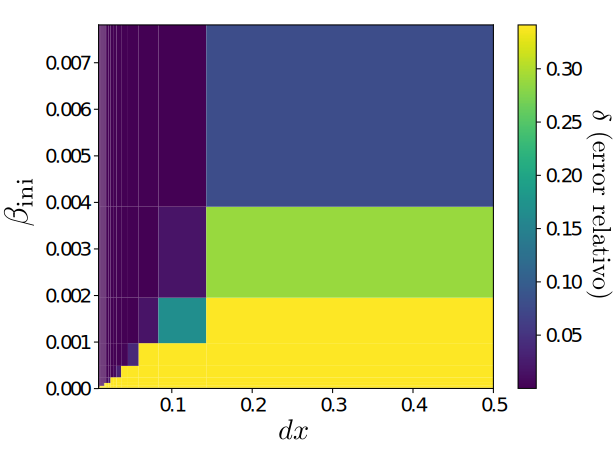
\includegraphics[width=\linewidth]{{{figures/pi_x-ms-opt-plot-harmonic_potential-beta_fin_4.000-x_max_5.000-nx_min_20-nx_max_1121-nx_sampling_50-N_iter_min_9-N_iter_max_20}}}
	\caption{Error relativo cuantificado por (\ref{eq:Msq-err-comp}) para $\beta_\mathrm{fin}=4$. Notamos que cuanto más pequeña sea $\beta_\mathrm{ini}$, la discretización $dx$ debe disminuir también para evitar que el error computacional sea grande.}
	\label{fig:Msq-err-comp}  
\end{figure}

En la figura \ref{fig:Msq-err-comp} mostramos los valores de el error relativo $\delta$ para $\beta_\mathrm{fin}=4$ al variar los parámetros $dx$ y $\beta_\mathrm{ini}$. Encontramos acá un comportamiento en cierta medida esperado: si se escogen valores de temperatura inversa inicial $\beta_\mathrm{ini}$ lo suficientemente pequeños en conjunto con espaciamientos $dx$ lo suficientemente pequeños, el error computacional es pequeño. Esto tiene sentido, ya que en estos límites la discretización es más suave (se parece más a un continuo) y la aproximación de Trotter se hace más 'válida' ya que la temperatura inicial es mayor. El valor que se paga por tomar estos valores pequeños es tiempo computacional, que en este caso no se reporta, pero es significativamente mayor cuanto más pequeña es la discretización $dx$ (asumiendo que $x_\mathrm{max}$ se deja constante). 

Notamos también que cuanto más pequeño queramos que sea $\beta_\mathrm{ini}$, necesitamos un valor de discretización aún más pequeño para que el error computacional no sea grande. Esto se debe a que en el momento de construir la figura nos encontramos con que hay unos valores de los parámetros $dx$ y $\beta_\mathrm{ini}$ para los cuales el algoritmo no converge a una respuesta, es decir, los valores de $\pi^{(Q)}_\mathrm{comp}(x ; \beta_\mathrm{fin})$ daban $\mathrm{nan}$ ó $\mathrm{inf}$, lo cual implica que el error en estos casos sería `infinito'. Sin embargo, en la gráfica lo que se asignó a estos valores fue el error máximo que se encontró en esta región, excluyendo los valores para los cuales el algoritmo no convergió a una respusta (en este caso color amarillo). Se hizo de esta manera para que la barra de colores pudiera dar cuenta de forma acertada de todos los errores en la región de $dx$ y $\beta_\mathrm{ini}$ escogida. De lo contrario, lo que se visualizaría en la gráfica sería solo color amarillo totalmente en las regiones que no convergía el algoritmo y  azul totalmente en las regiones en que si convergía y los valores intermedios no se hubiesen podido visualizar. En términos prácticos, la región que está pintada en amarillo en el gráfico indica que el algoritmo no converge para los parámetros dados allí y esto se debe a que la precisión computacional no es suficiente para resolver el problema.

\begin{figure}[!ht]
	\centering
	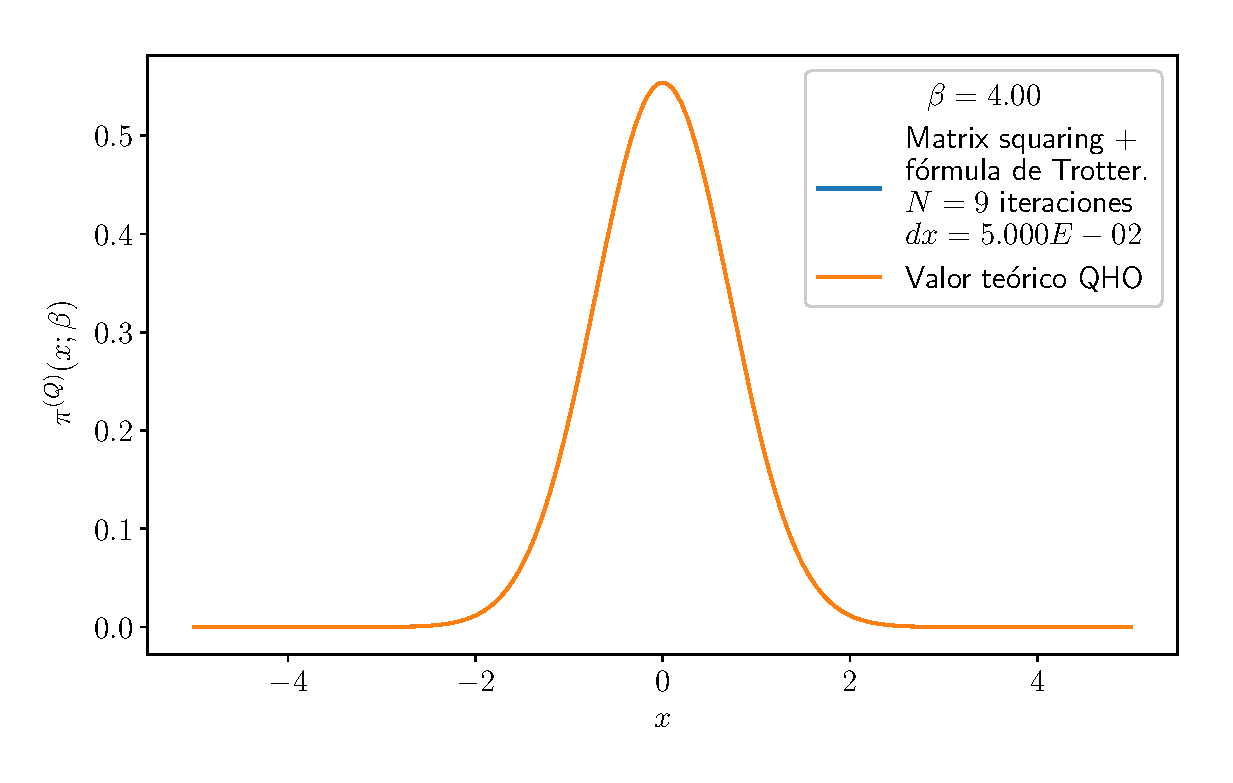
\includegraphics[width=\linewidth]{{{figures/pi_x-ms-plot-harmonic_potential-beta_fin_4.000-x_max_5.000-nx_201-N_iter_9}}}
	\caption{$\pi^{(Q)}_\mathrm{teo}(x ; \beta_\mathrm{fin})$ y $\pi^{(Q)}_\mathrm{comp}(x ; \beta_\mathrm{fin})$ para el oscilador armónico cuántico. En la gráfica solo aparece uno de los valores ya que el error computacional en este caso fue muy pequeño y las gráficas se solaparon. Los parámetros del algoritmo fueron $\beta_\mathrm{fin} = 4$, $\beta_\mathrm{ini} = 2^{-9}\beta_\mathrm{fin}$, $x_\mathrm{max}=5$, $dx=0.05$.}
	\label{fig:Msq-harm}
\end{figure}

Para obtener $\pi^{(Q)}_\mathrm{comp}(x ; \beta_\mathrm{fin})$ con $\beta_\mathrm{fin}=4$ nos basamos en la figura \ref{fig:Msq-err-comp} para escogier los parámetros $dx=0.05$ y $\beta_\mathrm{ini} = 2^{-9}\beta_\mathrm{fin}\approx0.0078$, que como vemos en la figura mencionada, tiene un error apreciablemente pequeño, además no toma tanto tiempo computacional. Con los parámetros mencionados se construyó la figura \ref{fig:Msq-harm} que en principio muestra tanto el valor teórico como el computacional de $\pi^{(Q)}(x;\beta)$. Las diferencias entre $\pi^{(Q)}_\mathrm{teo}(x ; \beta_\mathrm{fin})$ y $\pi^{(Q)}_\mathrm{comp}(x ; \beta_\mathrm{fin})$ son tan pequeñas, que en la gráfica están solapadas completamente y solo se alcanza a ver una de ellas. Con este resultado notamos que los parámetros escogidos están bien optimizados y nos sirve para calibrar estos parámetros para el oscilador anharmónico

\begin{figure}[!ht]
	\centering
	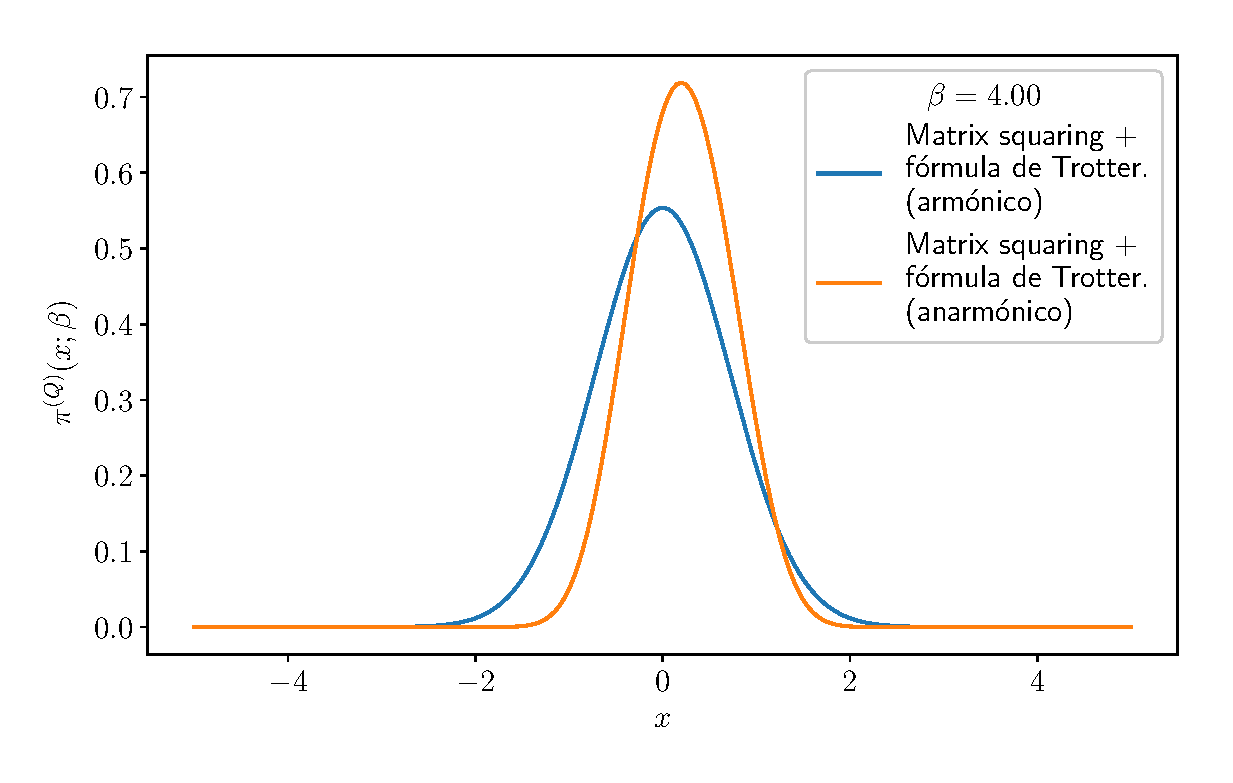
\includegraphics[width=\linewidth]{{{figures/pi_x-ms-plot-compare_potential-beta_fin_4.000-x_max_5.000-nx_201-N_iter_9}}}
	\caption{$\pi^{(Q)}_\mathrm{comp}(x ; \beta_\mathrm{fin})$ para el potencial anarmónico (\ref{eq:anharm-pot}). Se muestra también para comparación $\pi^{(Q)}_\mathrm{comp}(x ; \beta_\mathrm{fin})$ del potencial armónico. Los parámetros del algoritmo fueron $\beta_\mathrm{fin} = 4$, $\beta_\mathrm{ini} = 2^{-9}\beta_\mathrm{fin}$, $x_\mathrm{max}=5$, $dx=0.05$.}
	\label{fig:Msq-anharm}
\end{figure}

La figura \ref{fig:Msq-anharm} muestra el valor de $\pi^{(Q)}_\mathrm{comp}(x ; \beta_\mathrm{fin})$ para el potencial anarmónico
\begin{equation}
	V(x) = \frac{1}{2}x^2 - x^3 + x^4, \label{eq:anharm-pot}
\end{equation}
y se muestra también para comparar el resultado para el potencial armónico. Notamos que la forma de general la curva es muy similar a la del oscilador anharmónico. Sin embargo, se nota la asimetría del potencial anarmónico, ya que hay un corrimiento hacia la derecha con respecto al armónico. También vemos que para el potencial anarmónico es más angosto el pico, esto se deduce ya que su altura es máyor a comparación con el potencial armónico.

\begin{figure}[!ht]
	\centering
	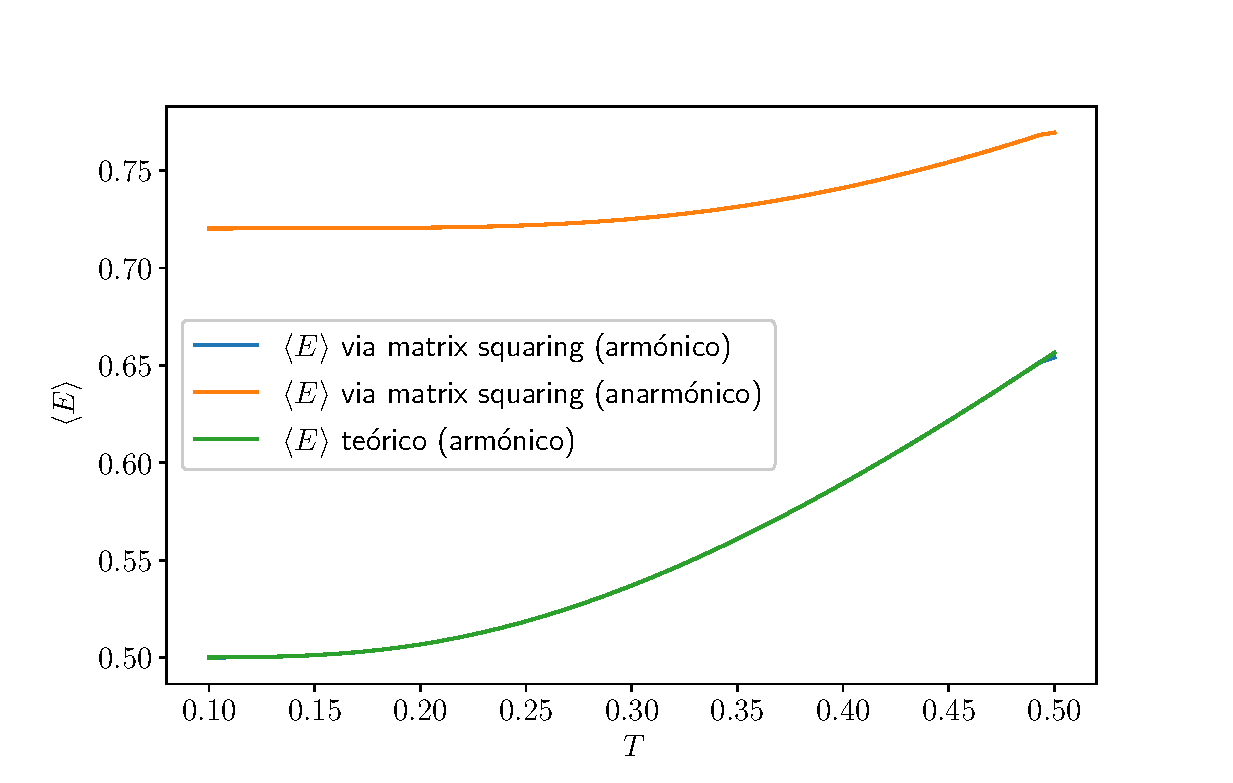
\includegraphics[width=\linewidth]{{{figures/E-ms-plot-compare_potential-beta_max_10.000-beta_min_2.000-N_temp_300-x_max_5.000-nx_201-N_iter_9}}}
	\caption{$\langle E \rangle$ dada por (\ref{eq:Energ-prom}) y calculada usando las matrices obtenidas mediante algoritmo \textit{Matrix Squaring} para los potenciales armónico y anharmónico. Los parámetros usados fueron $\beta_\mathrm{ini} = 2^{-9}\beta_\mathrm{fin}$, $x_\mathrm{max}=5$, $dx=0.05$. Se notan diferencias entre el valor teórico y el computacional para el potencial armónico pero solo en las puntas por el efecto de la derivada numérica en los extremos. Notamos que para el potencial armónico el límite de $T \rightarrow 0$ corresponde con el de la energía base $E=1/2$, mientras que el caso del potencial anarmónico la energía en este límite es un poco myor. La forma de las curvas para el potencial anarmónico y el armónico son similares.}
	\label{fig:E-msq}
\end{figure}

Con este mismo algoritmo es posible encontrar la función partición para diferentes valores de beta, ya que
\begin{equation}
	Z(\beta) = \int dx \rho(x,x;\beta).
\end{equation}
Con la ayuda de ésta se puede calcular a su vez el valor de la energía promedio del sistema mediante la conocida relación
\begin{equation}
	\langle E \rangle=-\frac{\partial}{ \partial \beta} \ln Z.
\end{equation}

En la figura \ref{fig:E-msq} se muestra la energía promedio para diferentes valores de temperatura cercanos a $T=0$, tanto para el potencial armónico, como para el potencial anarmónico. Además, se muestra el valor teórico para el potencial armónico
\begin{equation}
	\langle E \rangle = \frac{1}{2}\coth(\beta/2). \label{eq:Energ-prom}
\end{equation}
Encontramos que el calculo computacional de $\langle E \rangle$ para el potencial armónico está casi totalmente solapado con su contraparte teórica. Los errores apreciables están en las puntas de la gráfica y son debidos a efectos normales por cálculo numérico de la derivada en los extremos, que es más imprecisa que en la mitad de la gráfica. Notamos también que en el límite $T \rightarrow 0$, $\langle E \rangle\rightarrow 1/2$, tal y como se espera, ya que a temperatura cero el sistema tiende al estado base que en este caso tiene energía $E = 1/2$.

En el caso del cálculo computacional de  $\langle E \rangle$ para el potencial anarmónico, vemos que el límite $T \rightarrow 0$ la energía es un poco mayor que para el caso del potencial armónico, es decir, se espera que la energía del estado base del oscilador anarmónico sea mayor y coincida con el límite que se muestra en esta gráfica. También notamos que en temperaturas cercanas a cero, la energía cambia más lentamente que cuando se compara con la gráfica del potencial armónico. Sin embargo, tal y como se espera, el comportamiento de $\langle E \rangle$ no es muy diferente al del oscilador en este límite de `bajas' temperatiuras.

Nota: los programas de Python3 en los que se implementó este algoritmo y con los que se realizaron estas gráficas se pueden encontrar en el apéndice \ref{appx:codigo_matrix_squaring}. 

\subsection{\textit{Path Integral Naive Sampling}\label{subsec:PathInt-results}}


Para este algoritmo, el camino que se cambiará en cada iteración consta de diez posiciones. Es decir, en (\ref{eq:path-ini}) se toma $N=10$. Además se tomó $\delta = 0.5$ y el número de iteraciones que se hicieron fue $N_\mathrm{iter}=10^6$.

\begin{figure*}[!ht]
	\centering
	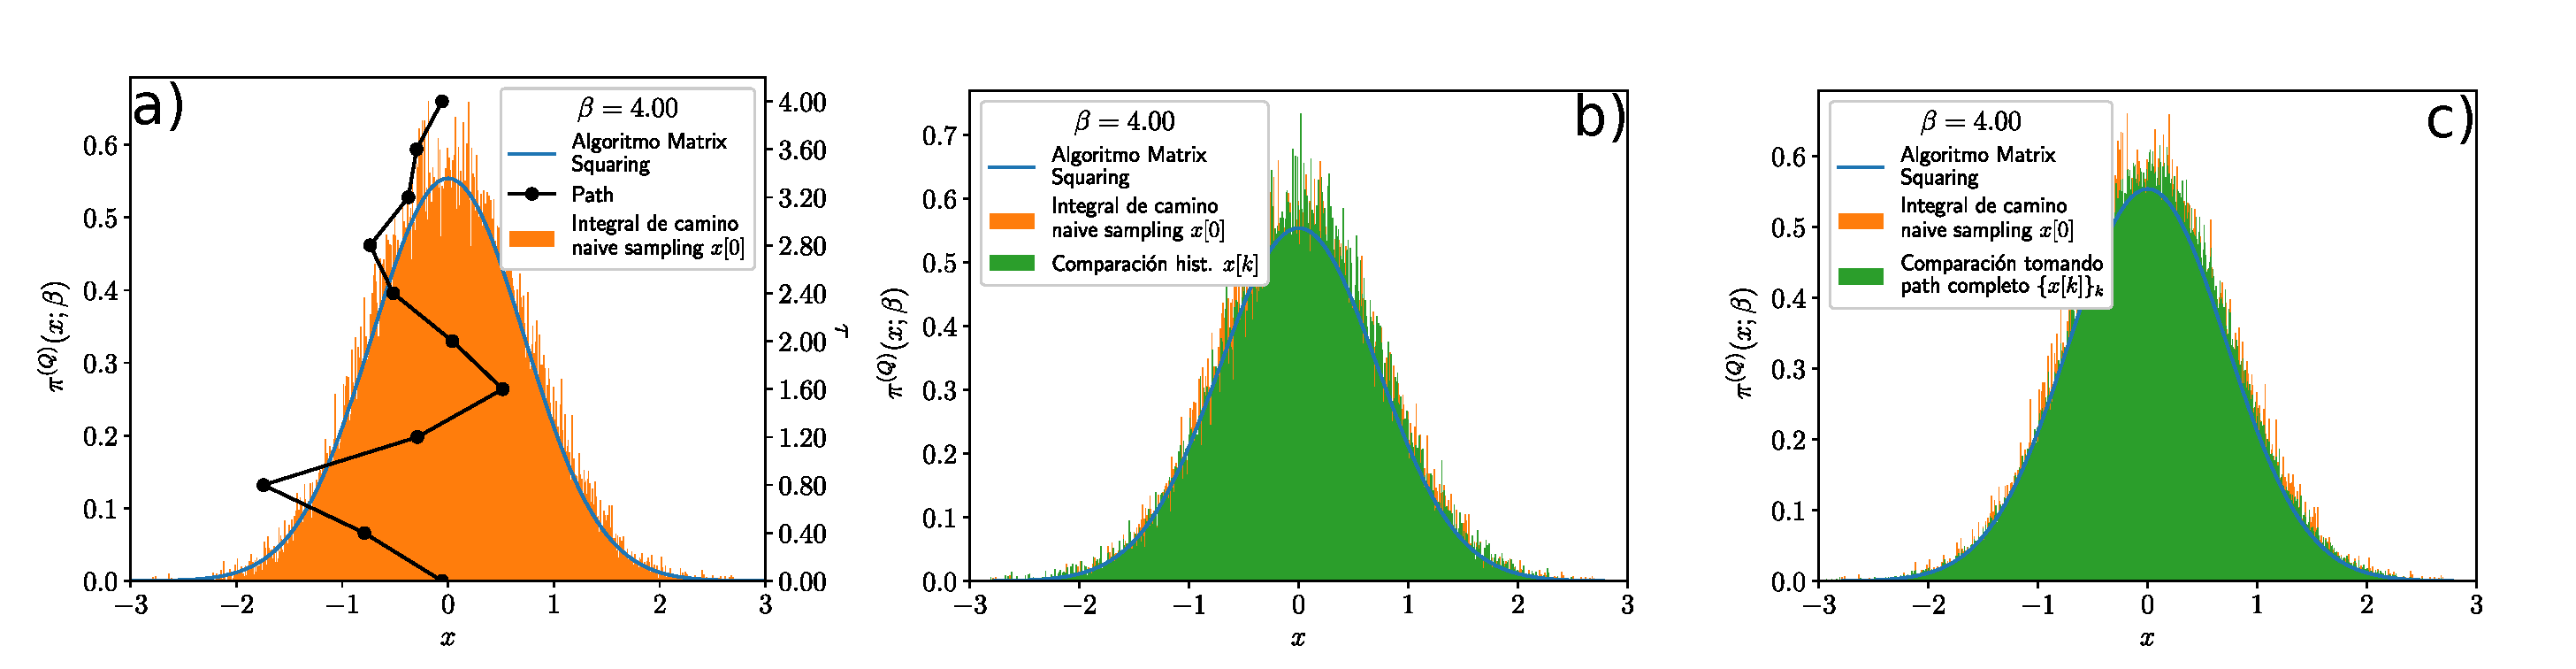
\includegraphics[width=\linewidth]{{{figures/pi_x-pi-plots-harmonic_potential-beta_4.000-N_path_10-N_iter_1000000-delta_0.500-append_every_1-x_max_3.000}}}
	\caption{Histogramas para el potencial armónico obtenidas con el algoritmo \textit{Path Integral Naive Sampling}. a) Histograma para posiciones $x_0$; semuestra también el path que se obtiene al final del algoritmo. b) Histograma para posiciones $x_0$ y comparación con histograma para $x_k$ con $k\neq0$ notamos que los histogramas coinciden en la forma y se ajustan al los valores dados por el algoritmo \textit{Matrix Squaring}. c) Histograma para posiciones $x_0$ y comparación con histograma generado por los valores que toma todo el camino $[x_0,\,\,x_1,\,\,\dots,\,\,x_{9}]$. Si se hace Zoom en éste último y se compara con los otros, podemos ver que las fluctuaciones alrededor del valor teórico disminuyen debido a que acá se consideran más datos. Los parámetros usados para este caso fueron $N_\mathrm{iter}=10^6$ y $\delta=0.5$.}
	\label{fig:path-int-harm}
\end{figure*}

En la figura \ref{fig:path-int-harm} encontramos los resultados para el potencial armónico. En la figura a) vemos el histograma tomando solo las posiciones $x_0$ de  $X$ (\ref{eq:path-ini}) que se guarda en cada iteración. Además podemos ver allí también el resultado del algoritmo \textit{Matrix Squaring} que se muestra como línea continua (el eje y correspondiente a estos datos es el de la izquierda). Podemos ver que los resultados del algoritmo \textit{Path Integral Naive Sampling} se ajustan en términos generales a la forma del resultado del algoritmo \textit{Matrix Squaring} (que en este caso en términos prácticos es idéntico al teórico). Notamos sin embargo que hay bastantes fluctuaciones en los resultados del histograma, lo cual está muy relacionado con el hecho de que es un algoritmo tipo Montecarlo que depende de números aleatorios. Es probable que si se aumenta significativamente el número de iteraciones se logren disminuir las fluctuaciones. También esto puede estar relacionado con el número de \textit{bins} que se usaron que fue $\sqrt{N_\mathrm{iter}}$, que es una regla usada comunmente. Lo interesante de usar bastantes \textit{bins} es que precisamente estas fluctuaciones son evidentes y notamos que el algoritmo no ha convergido totalmente al resultado esperado y que son necesarias más iteraciones para obtener punto a punto un resultado más cercano al teórico y no solo la forma general. Por el aumento de tiempo computacional no se intentó realizar un número significativamente mayor de iteraciones, pero en principio el algoritmo debe converger a la solución, tal como podemos intuir a partir del resultado obtenido con el valor de $N_\mathrm{iter}$ escogido. En esta misma figura a) encontramos también el camino $X=[x_0,\,\,x_1,\,\,\dots,\,\,x_{9}]$ que resulta al final de las $10^6$ iteraciones. Es interesante ver que los valores por los que pasa el camino se ubican predominantemente entre $x=-1$ y $x=1$, esto en conformidad con la región de mayor probabilidad, de acuerdo con lo que vemos en el histograma el eje y para este camino es el de la derecha, que marca los valores de $\beta$ para cada paso del camino, segun se acostumbra graficar.

En la figura \ref{fig:path-int-harm}c) podemos ver el histograma construido con la unión de todos los caminos por los que pasó el algoritmo y en  la figura \ref{fig:path-int-harm}b) podemos ver el histograma construido con los valores de $x_k$ con $k \neq 0$. En los dos casos vemos que el histograma coincide en términos generales con el mostrado en la figura \ref{fig:path-int-harm}a), que se muestra también en las figuras mencionadas para comparación. Hay un detalle sutil que hace diferencia en estos dos histogramas y es que cuando se construye con el camino completo (es decir, el que se muestra en \ref{fig:path-int-harm}c)) las fluctuaciones disminuyen. Esto se puede ver haciendo zoom en ambas figuras b) y c) y es debido a que en la figura c) por tratarse del camino completo, estamos teniendo en cuenta $10^7$ posiciones y no $10^6$ (el cual es el caso de las otras dos figuras). Al ser construido con más datos, las fluctuaciones alrededor del valor teórico disminuyen un poco.

Por otro lado en las figuras \ref{fig:path-int-anharm} encontramos las figuras análogas al caso anterior pero acá para el potencial anarmónico. Encontramos en términos generales que las características de estas figuras son muy similares a las del caso armónico. Las diferencias obvias son que este histograma está más corrido hacia la derecha, lo cual refleja el hecho de que este potencial es asimétrico con respecto al eje $x=0$. Igualmente, en este caso se nota que las fluctuaciones disminuyen un poco cuando se considera el camino completo.

\begin{figure*}[!ht]
	\centering
	\includegraphics[width=\linewidth]{{{figures/pi_x-pi-plots-anharmonic_potential-beta_4.000-N_path_10-N_iter_1000000-delta_0.500-append_every_1-x_max_3.000}}}
	\caption{{Histogramas para el potencial anararmónico (\ref{eq:anharm-pot}) obtenidas con el algoritmo \textit{Path Integral Naive Sampling}. a) Histograma para posiciones $x_0$; semuestra también el path que se obtiene al final del algoritmo. b) Histograma para posiciones $x_0$ y comparación con histograma para $x_k$ con $k\neq0$ notamos que los histogramas coinciden en la forma y se ajustan al los valores dados por el algoritmo \textit{Matrix Squaring}. c) Histograma para posiciones $x_0$ y comparación con histograma generado por los valores que toma todo el camino $[x_0,\,\,x_1,\,\,\dots,\,\,x_{9}]$. Si se hace Zoom en éste último y se compara con los otros, podemos ver que las fluctuaciones alrededor del valor teórico disminuyen debido a que acá se consideran más datos. Los parámetros usados para este caso fueron $N_\mathrm{iter}=^6$ y $\delta=0.5$.}}
	\label{fig:path-int-anharm}
\end{figure*}



Como comentario final de esta sección, es importante también mencionar que los algoritmos se ejecutaron en Python3 v3.6.

\section{Conclusión\label{sec:conclusion}}

En este trabajo estudiamos el problema del oscilador armónico en un baño térmico, bajo un efoque computacional a la luz de los algoritmos \textit{Matrix Squaring} y \textit{Path Integral Naive Sampling}.

En el caso del primer algoritmo notamos que es robusto y los resultados para el potencial armónico coinciden con los valores teóricos. En este algoritmo pudimos implamentar una optimización para los parámetros $\beta_\mathrm{ini}$ y $dx$ y encontramos que cuanto más pequeño sea $\beta_\mathrm{ini}$, más pequeña debe ser la discretización $dx$ para evitar errores computacionales. Se encontraron diferencias evidentes para $pi^{(Q)}(x;\beta)$ entre el potencial armónico y el anarmónico, la más evidente es el desplazamiento del pico para el anarmónico hacia la derecha. Sin embargo, si solo se mira la forma de las curvas ambas son muy similares, aunque la del anarmónico tiene el pico con una densidad de probabilidad mayor. Acá también encontramos que los valores obtenidos para la energía promedio $\langle E \rangle$ coinciden con los teóricos y en el caso del oscilador armónico, el límite de baja temperatura coincide con la energía del estado base del sistema $E=1/2$, mientras que para el potencial anarmónico la energía en este límite fue un poco más grande. Sin embargo, de nuevo, el comportamiento de la curva en su forma es similar para los dos casos.

En el caso del segundo algoritmo, encontramos que no es tan preciso como el primero pero es un método valioso para contrastar y corroborar los resultados que se obtuvieron. Encontramos que cuando se tiene en cuenta el camino completo para graficar el histograma, las fluctuaciones alrededor del valor teórico dismiuyeron un poco y esperamos que si se incrementa significativamante $N_\mathrm{iter}$, estas fluctuaciones disminuyan aún más. Para los caminos graficados, tanto en el caso anarmónico como en el armónico, encontramos que los valores de las pociciones se concentran en las regiones de mayor probabilidad. 

Para trabajos futuros sería interesante evaluar en más detalle el papel que juega el número de iteraciones en cada algoritmo así como el número de posiciones considerado para los caminos en el algoritmo de \textit{Path Integral Naive Sampling}.

Las implementaciones de los algoritmos usados en este trabajo son suficientemente generales y se podrían adaptar con cierta facilidad a otros sistemas de interés que sean objeto de estudio.

\section*{Agradecimientos}
Agradezco a mis compañeros de clase con los que tuve discusiones que ayudaron en la implementación del algoritmo y en las conclusiones presentadas.

\nocite{*}

\bibliography{5-Semestre_X_2020_I-Fisica_Estadistica_Avanzada-Tarea_2}% Produces the bibliography via BibTeX.

\newpage



\appendix

\begin{widetext}

\section{Código 1: Matrix Squaring\label{appx:codigo_matrix_squaring}}

A continuación se muestra el código que corre los algoritmos que se usaron para la parte de Matrix Squaring en la sección \ref{subsec:Mtxsq-results}. Éste código usa el módulo matrix\_squaring que está disponible en \href{https://github.com/jearistiz/Statistical-Physics-Projects/blob/master/2/matrix_squaring.py}{este link}. Cada función del módulo está comentada y explicada.

\inputminted[linenos,breaklines]{python}{code_1.py}

\section{Código 2: Naive Path Integral Montecarlo Sampling\label{appx:codigo-path-int}}

A continuación se muestra el código que corre los algoritmos que se usaron para la parte de \textit{Path Integral Naive Sampling} en la sección \ref{subsec:PathInt-results}. Éste código usa el módulo path\_integral\_naive\_sampling que está disponible en \href{https://github.com/jearistiz/Statistical-Physics-Projects/blob/master/2/path_integral_naive_sampling.py}{este link}. Cada función del módulo está comentada y explicada.

\inputminted[linenos,breaklines]{python}{code_2.py}

\end{widetext}


\end{document}
%
% ****** End of file apssamp.tex ******
